\newcommand{\seccion}{SECUNDARIA INCORPORADA A LA SEG }
\newcommand{\descripcion}{Repaso Bimestral, Segundo Bimestre }
\newcommand{\grado}{Primero de secundaria}
\newcommand{\ciclo}{Ciclo escolar: 2015--2016}
\newcommand{\papel}{legalpaper} %letterpaper, legalpaper ...
\newcommand{\fecha}{5 de diciembre de 2015}

\author{M. en C. Reinaldo Zapata}

\documentclass[11pt]{article}
\usepackage[\papel]{geometry}

\title{\flushleft \seccion \\ \descripcion \\  \grado \\ \ciclo}

\newcommand\BackgroundLogo{
\put(162,365){
\parbox[b][\paperheight]{\paperwidth}{%
\vfill
\centering
\includegraphics[width=5cm,height=2.5cm,keepaspectratio]{/Users/reinaldo/Documents/clases/jassa/logo}%
\vfill
}}}

% \hyphenation{con-ti-nua-ci\'on}

\usepackage{enumitem}
\usepackage[T1]{fontenc} %fuentes
\usepackage{lmodern} %fuente mejorada
\usepackage[spanish]{babel}
\decimalpoint
\usepackage{fullpage}
\usepackage{multicol}
\usepackage{graphicx}
\usepackage{eso-pic}
\usepackage{multirow}
\usepackage{subfigure}
\usepackage{tikz}
\usepackage{hyperref} 
\usepackage{color}
\usepackage{multicol}
\usepackage{tikz}
\usetikzlibrary{shapes.geometric}



\usepackage[leqno,fleqn]{amsmath}
\makeatletter
  \def\tagform@#1{\maketag@@@{#1\@@italiccorr}}
\makeatother
\renewcommand{\theequation}{\fbox{\textbf{\arabic{equation}}}}


\begin{document}
\AddToShipoutPicture*{\BackgroundLogo}
\ClearShipoutPicture
\date{7 de diciembre de 2015}
\maketitle

Nombre del alumno:\,\line(1,0){244}\,.\hspace*{.2cm} No. de lista:\,\line(1,0){35}\,.

Primero de secundaria, grupo:\,\line(1,0){30}\,.

\vspace{5mm}

El prop\'osito de esta gu\'ia de estudio es proporcionar al alumno un repaso de
los temas que ser\'an vistos en el examen bimestral. Contesta de forma correcta
cada uno de los reactivos que se muestran a continuaci\'on. Escribe las
respuestas en esta hoja de estudio y entrega por separado las operaciones
correspondientes.

\section{Fracciones y decimales}

Convierte cada fracci\'on a decimal y viceversa. Simplifica tus resultados si es
posible.

\begin{multicols}{4}

\begin{equation} \frac{3}{4} =    \end{equation}
\begin{equation} \frac{15}{64} =  \end{equation}
\begin{equation} \frac{21}{25} =  \end{equation}
\begin{equation} 0.23 =           \end{equation}
\begin{equation} 0.049 =          \end{equation}
\begin{equation} 9.275 =          \end{equation}
\begin{equation} 4\frac{5}{16} =  \end{equation}
\begin{equation} \frac{14}{75} =  \end{equation}
\begin{equation} \frac{17}{100} = \end{equation}
\begin{equation} 0.875 =          \end{equation}
\begin{equation} 3.75 =           \end{equation}
\begin{equation} 3.1416 =         \end{equation}

\end{multicols}

\vspace{5mm}

Resuelve las siguientes operaciones con fracciones.
\begin{multicols}{2}
\begin{align}
\left(  \frac{2}{3} + \frac{2}{15} \right) \div \frac{1}{6} = \\
\left( 16 + \frac{3}{4} \div 4\frac{3}{5} \right) = \\
\left( 4 - \frac{2}{3} \div \frac{11}{16} \right) = 
\end{align}

\begin{align}
\frac{13}{5} \div \left( \frac{2}{9} + \frac{5}{18} \right) =\\
\frac{9}{5} \div \left( 4\frac{2}{6} - 1\frac{3}{12} \right) = \\
\left( \frac{5}{2} + \frac{3}{4} - \frac{1}{8} \right) \div 1\frac{8}{5} = 
\end{align}
\end{multicols}

\vspace{0.5cm}

Resuelve las siguientes operaciones con decimales.

\begin{multicols}{2}
\begin{align}
(4.5 + 8)(3.4) = \\
(6.7 - 2) \div (9 - 7.5) = \\
7 + 11 \times 6.5 = 
\end{align}

\begin{align}
(3 \div 5) \times (7 - 1.017) = \\
(9 + 4.545 - 4) \times (12 - 1.85) \div 2 = \\
(12 + 4.545 - 6) \times (18 - 10.85) \div 3.1 = 
\end{align}
\end{multicols}

\newpage

\subsection{Problemas}

A una contenedor de aceite industrial de $\frac{3}{4}$ de metro c\'ubico se le
extrae $\frac{1}{5}$ de su capacidad. ?`Qu\'e fracci\'on de su contenido queda?

\vspace{1cm}

Un pescador vendi\'o $\frac{1}{6}$ del total de su pesca, $\frac{1}{3}$ 
de la misma la entreg\'o en el mercado, guard\'o $\frac{1}{4}$ para su familia y
el resto lo don\'o a un albergue. ?`Qu\'e fracci\'on de la pesca don\'o?

\vspace{1cm}

Un corredor entrena recorriendo distintas distancias cada d\'ia. El primero
recorri\'o 10\,Km, el segundo corri\'o 6.3\,Km y el tercero corri\'o 12\,Km.
?`Qu\'e distancia recorri\'o en total durante estos tres d\'ias? ?`Cu\'anto le
falta para recorrer un total de 40\,Km?

\vspace{1cm}

\section{Rectas num\'ericas}

Usando la recta que se muestra a continuaci\'on coloca en el extremo izquierdo
el n\'umero cero (0) y en el extremo derecho el n\'umero dos (2). Usando esa
misma recta ubica las siguientes cantidades:
\begin{multicols}{5}
\begin{enumerate}[label=\alph*)] \itemsep-.3em
\item $\displaystyle\frac{4}{5} $ \hspace{5mm} 
\item 0.9 
\item 0.6 
\item 1.1
\item $\displaystyle\frac{11}{6} $
\end{enumerate}
\end{multicols}

\vspace{5mm}

\begin{centering}

\begin{tikzpicture}
\draw [thick,color=black] (0,0)--(10,0);
\end{tikzpicture}

\end{centering}

\vspace{5mm}

En un circuito de 10 kil\'ometros se realiz\'o una carrera de ciclistas. Los
competidores comenzaron en el punto de partida (punto ``A'') en direcci\'on
hacia la derecha, como se muestra en la figura a continuaci\'on. Algunos de los
corredores tuvieron accidentes en distintas secciones. Ub\'icalas en la figura
correctamente.

\begin{minipage}{0.5\linewidth}
Puntos de accidentes: \hspace{3mm} 

\begin{enumerate}[label=\alph*)] \itemsep-.3em
\item $6\frac{2}{3}$\,Km, \hspace{3mm}
\item 4.5\,Km, \hspace{3mm} 
\item 3.1\,Km
\end{enumerate}

\end{minipage}%
\begin{minipage}{0.5\linewidth}

% \begin{figure}[h!]
    \begin{center}
        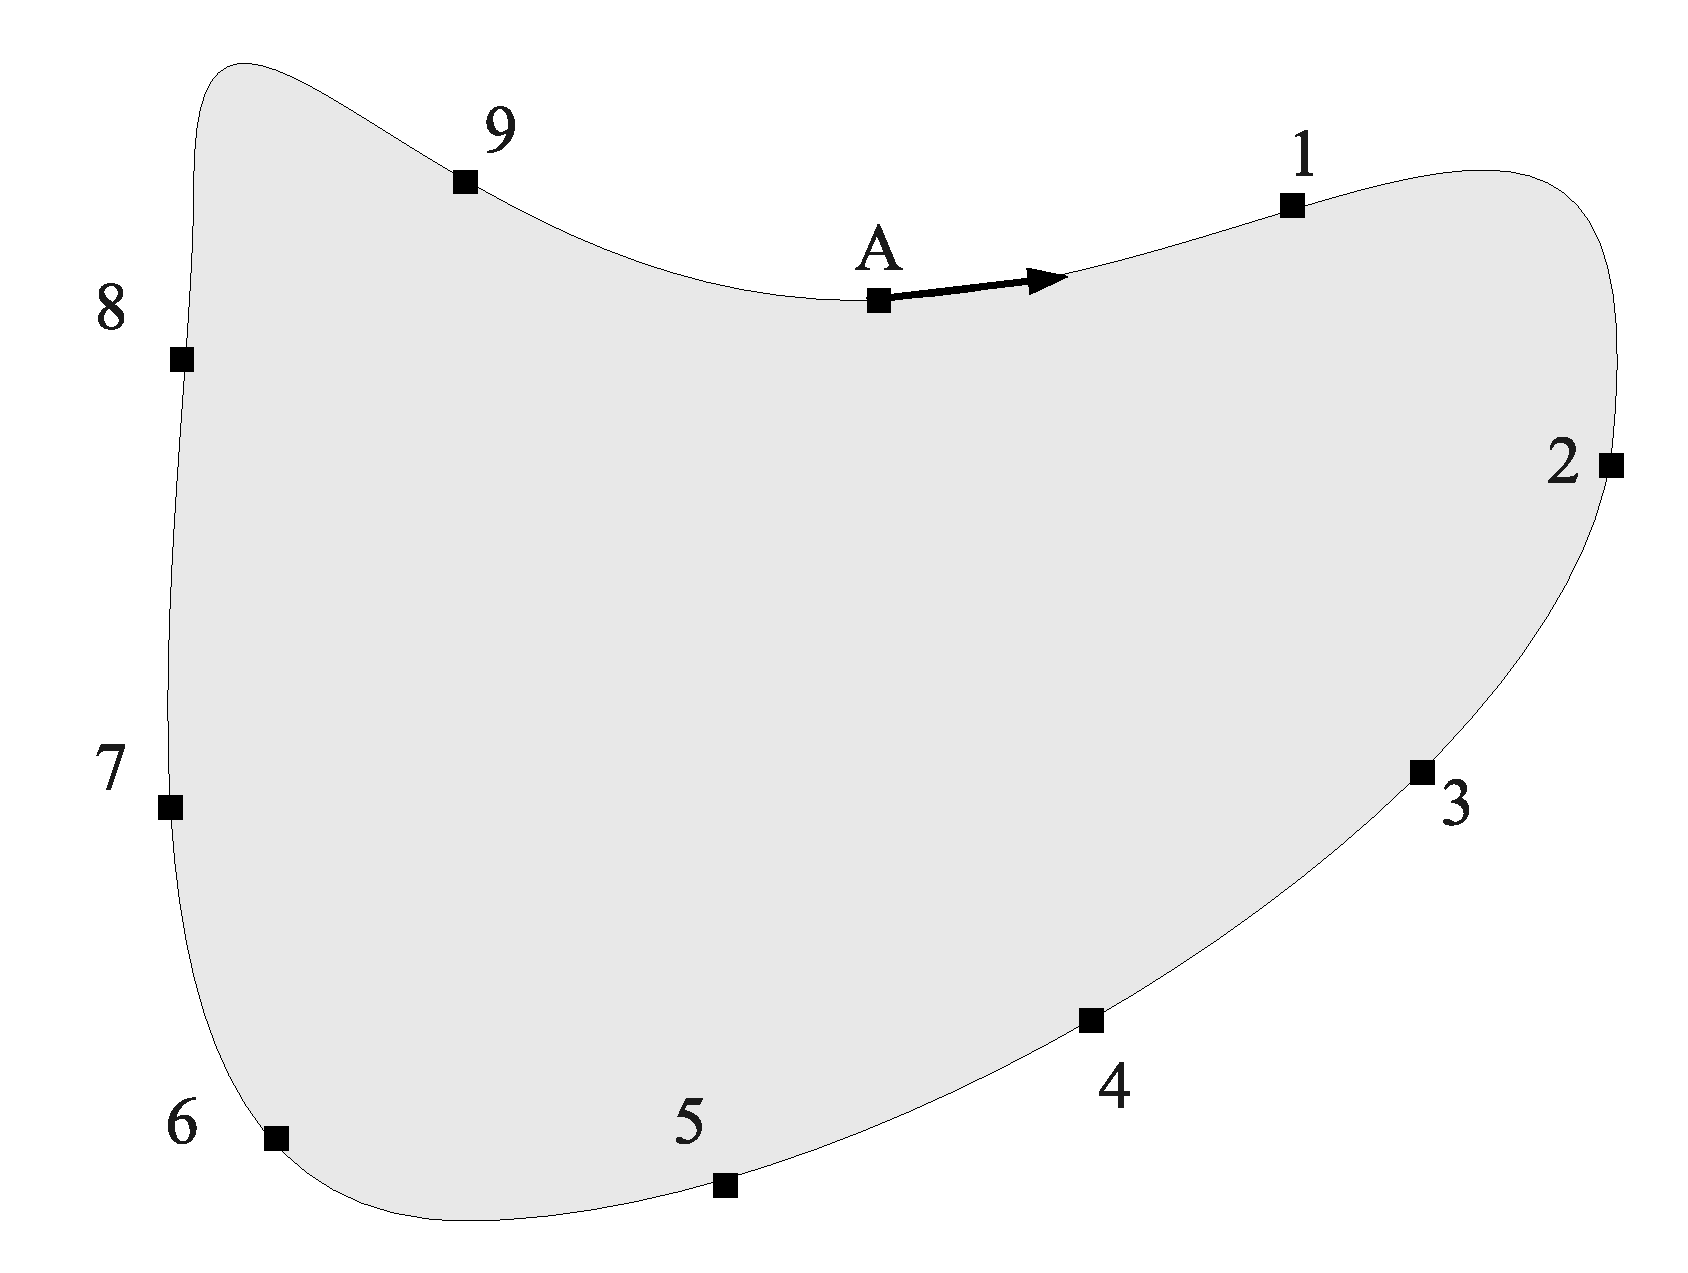
\includegraphics[width=0.8\textwidth]{pista}
    \end{center}
% \end{figure}
\end{minipage}

% \vspace{5mm}

\section{Probabiliad y estad\'istica}

En una bolsa hay un total de 30 canicas de las cuales cinco (5) son de
color amarillo, diez (10) son de color verde y el resto azules. Responde a las
siguientes preguntas:

\begin{enumerate}[label=\alph*)] \itemsep-.3em
\item ?`Qu\'e fracci\'on del total representan las canicas azules?
\item ?`Qu\'e fracci\'in decimal represntan las canicas amarillas?
\item ?`Qu\'e decimal representan las las canicas azules?
\item que decimal represntan las canicas verdes y azules juntas?
\end{enumerate}

\vspace{5mm}

Recuerda el experimento de lanzar dos dados. Acorde a ello responde para cada
inciso si la probabilidad de que suceda el evento es alta (\emph{A}), baja
(\emph{B}) o nula (0).

\begin{enumerate}[label=\alph*)] \itemsep-.3em
\item Que la suma de los n\'umeros en los dados sea 1.
\item Que la suma de los n\'umeros de los dados sea 6, 7 u 8.
\item Que la suma de los n\'umeros de los dados sea 2.
\item Que la suma de los n\'umeros de los dados sea un n\'umero mayor a 12.
\item Que la suma de los n\'umeros de los dados sea 12.
\end{enumerate}

Analiza el experimento de lanzar una moneda (no cargada) al aire en la que
puedes obtener como resultado cara o cruz. ?`Qu\'e es m\'as probable que caiga,
cara, cruz o la probabilidad es igual? Explica tu respuesta.

\vspace{3cm}

\section{Geometr\'ia}

\begin{multicols}{2}
% \setlength{\columnseprule}{0.4pt}
    
Traza un cuadrado que tenga 4\,cm de longitud lateral. Calcula su per\'imetro y
su \'area.

\vspace{5cm}
P=

A=

\vspace{1cm}

Traza un tr\'iangulo equil\'atero cuyo lado mide 3.5\,cm. Mide su altura y
m\'arcala. Calcula su per\'imetro y su \'area.

\vspace{5cm}
P=

A=

\vspace{1cm}

Traza un rect\'angulo que tenga como base 6\,cm y como altura 3\,cm.

\vspace{5cm}
P=

A=

\vspace{1cm}

Traza un rect\'angulo que tenga como base 6\,cm y como altura 3\,cm. Calcula su
per\'imetro y su \'area.

\vspace{5cm}
P=

A=

\vspace{1cm}

\end{multicols}
\begin{multicols}{2}

Traza un c\'irculo con rario $r=2.5$\,cm. Calculasu per\'imetro y su \'area.
\vspace{5cm}

P=

A=

\vspace{1cm}

Traza el esquema de un c\'irculo cuyo di\'ametro es 10\,m. Calcula su
per\'imetro y su \'area.

\vspace{5cm}
P=

A=

\vspace{1cm}

\end{multicols}


\begin{multicols}{2}

Mide la longitud lateral y el apotema del siguiene pent\'agono y coloca las
medidas donde correspnde. Calcula su per\'imetro y su \'area.

\begin{tikzpicture}[scale=2.2]%change the size here
\node [draw, thick, minimum size=5cm, regular polygon, regular polygon sides=5] at (0,0) { };
\draw [thick,color=black] (0,0.05)--(0,-0.05);
\draw [thick,color=black] (-0.05,0)--(0.05,0);
\draw [dashed, thick,color=black] (0,-0.9)--(0,0);
\node [right] at (0,-0.2) {a=};
\node [below] at (0,-0.9) {$\ell=$};
\end{tikzpicture}

\vspace{1cm}

P=

A=

Traza el apotema del siguiente hex\'agono. Mide su longitud lateral y el apotema
y escribe las medidas donde corresponde. Calcula su per\'imetro y su \'area.

\begin{tikzpicture}[scale=2]
\node [draw, thick, minimum size=5cm, regular polygon, regular polygon sides=6] at (0,0) { };
\draw [thick,color=black] (0,0.05)--(0,-0.05);
\draw [thick,color=black] (-0.05,0)--(0.05,0);
\node [right] at (0,-0.4) {a=};
\node [below] at (0,-1.1) {$\ell=$};
\end{tikzpicture}

\vspace{1cm}

P=

A=

\end{multicols}


\begin{multicols}{2}

Utilizando las l\'ineas que se muestran a continuaci\'on traza un tri\'angulo.
Recuerda usar el comp\'as. Traza su altura y calcula el per\'imetro y el \'area.

\vspace{5mm}

\begin{tikzpicture}[scale=2]
\draw [thick,color=black] (0,0)--(2,0);
\draw [thick,color=black] (0,0.5)--(1,0.5);
\draw [thick,color=black] (0,0.25)--(1.5,0.25);
\end{tikzpicture}

\vspace{6cm}


P=

A=

Traza un tri\'angulo is\'osceles utilizando como base la l\'inea que se muestra
a continuaci\'on. Usando el comp\'as haz que la medida de sus otros dos lados
sea $\ell_{1}=\ell_{2}=$\,6cm. Traza su altura y calcula su per\'imetro y su
\'area.


\begin{centering}
    
\vspace{5mm}

\begin{tikzpicture}
\draw [thick,color=black] (0,0)--(4,0);
\node [right] at (0,6) { };
\end{tikzpicture}

\end{centering}

P=

A=

\end{multicols}

\vspace{5mm}

Traza las mediatrices de los siguientes segmentos y la bisectriz de los
siguientes \'angulos.

\vspace{1cm}

\begin{centering}
\begin{tikzpicture}[scale=1.05]
\draw [thick,color=black] (0,2)--(4,0);
\draw [thick,color=black] (4,2)--(7,0); \draw [thick,color=black] (4,2)--(5,-1);
\draw [thick,color=black] (8,0)--(12,2);
\draw [thick,color=black] (11,-1)--(14,2); \draw [thick,color=black] (14,2)--(15,-1.2) ;
\end{tikzpicture}
\end{centering}



\end{document}

\left(  \right)




